\section{Introduction}
The main goal of this laboratory assignment is to analyse and better understand how an audio amplifier works and to design it having in mind that it should have a good relation efficiency-price. So, one has to find an optimal solution for the circuit built, which corresponds to a circuit that minimizes the cost, based not only in the number of component but on the type of them (see price table \ref{tab:price}), maximizing the amplifying bandwidth and minimizing the lower cutoff frequency. This is because the frequencies that are more difficult to achieve in a amplifier like the one analysed are the lower ones.\\

To calculate the total cost associated to this circuit, one considered that it equals the sum of the cost of the resistors, capacitors and transistors. This maximization process can be compacted in a function called merit.\\

\vspace{-2mm}
\begin{minipage}{.45\textwidth}
\begin{table}[H]
    \centering
    \begin{tabular}{c|c}
        \textbf{Component} &  \textbf{Price}\\
        \hline
        Resistors & 1 MU $k\Omega^{-1}$ \\
        Capacitors & 1 MU $\mu F^{-1}$ \\
        Transistors & 0.1 MU transistor$^{-1}$
    \end{tabular}
    \caption{Price table for the components used}
    \label{tab:price}
\end{table}
\end{minipage}
\begin{minipage}{.45\textwidth}
\begin{equation}
    M = \frac{10\log\left(\frac{V_{in}}{V_{out}}\right) * \text{bandwidth}}{\text{Cost}*\text{LowerCutOffFrequency}}
    \label{score}
\end{equation}
\end{minipage}\\\\

The bandwidth corresponds to the difference between the higher cutoff frequency and the lower cutoff frequency, and those being defined by the frequencies from which the gain is lower than 3dB compared with the maximum value obtained. The $V_{in}$'s maximum value is set at $10mV$ (mandatory) in order for the goal to be well defined. Additionally to the components seen in the price table \ref{tab:price}, we also use a voltage source of $12V$ that will have an important role in the amplification of the input voltage.\\

The circuit can also be divided in 2 main regions: the gain stage and the output stage. The gain stage has the main goal of amplifying the signal, as it is suggested by its name, and the output stage to reduce the impedance of the circuit that is connected to the output audio emitter of $8 \Omega$. This is necessary because having a high output impedance, Zo, in the circuit would make all the current pass through the audio emitter, wasting significant amounts of power and increasing the distortion of the signal. On the other hand, with the goal of averting the degradation of the input voltage, one must have a high input impedance, Zi\\

Furthermore, and considering all the points mentioned before, the circuit used for this purpose was the following:

\begin{figure}[H]
    \centering
    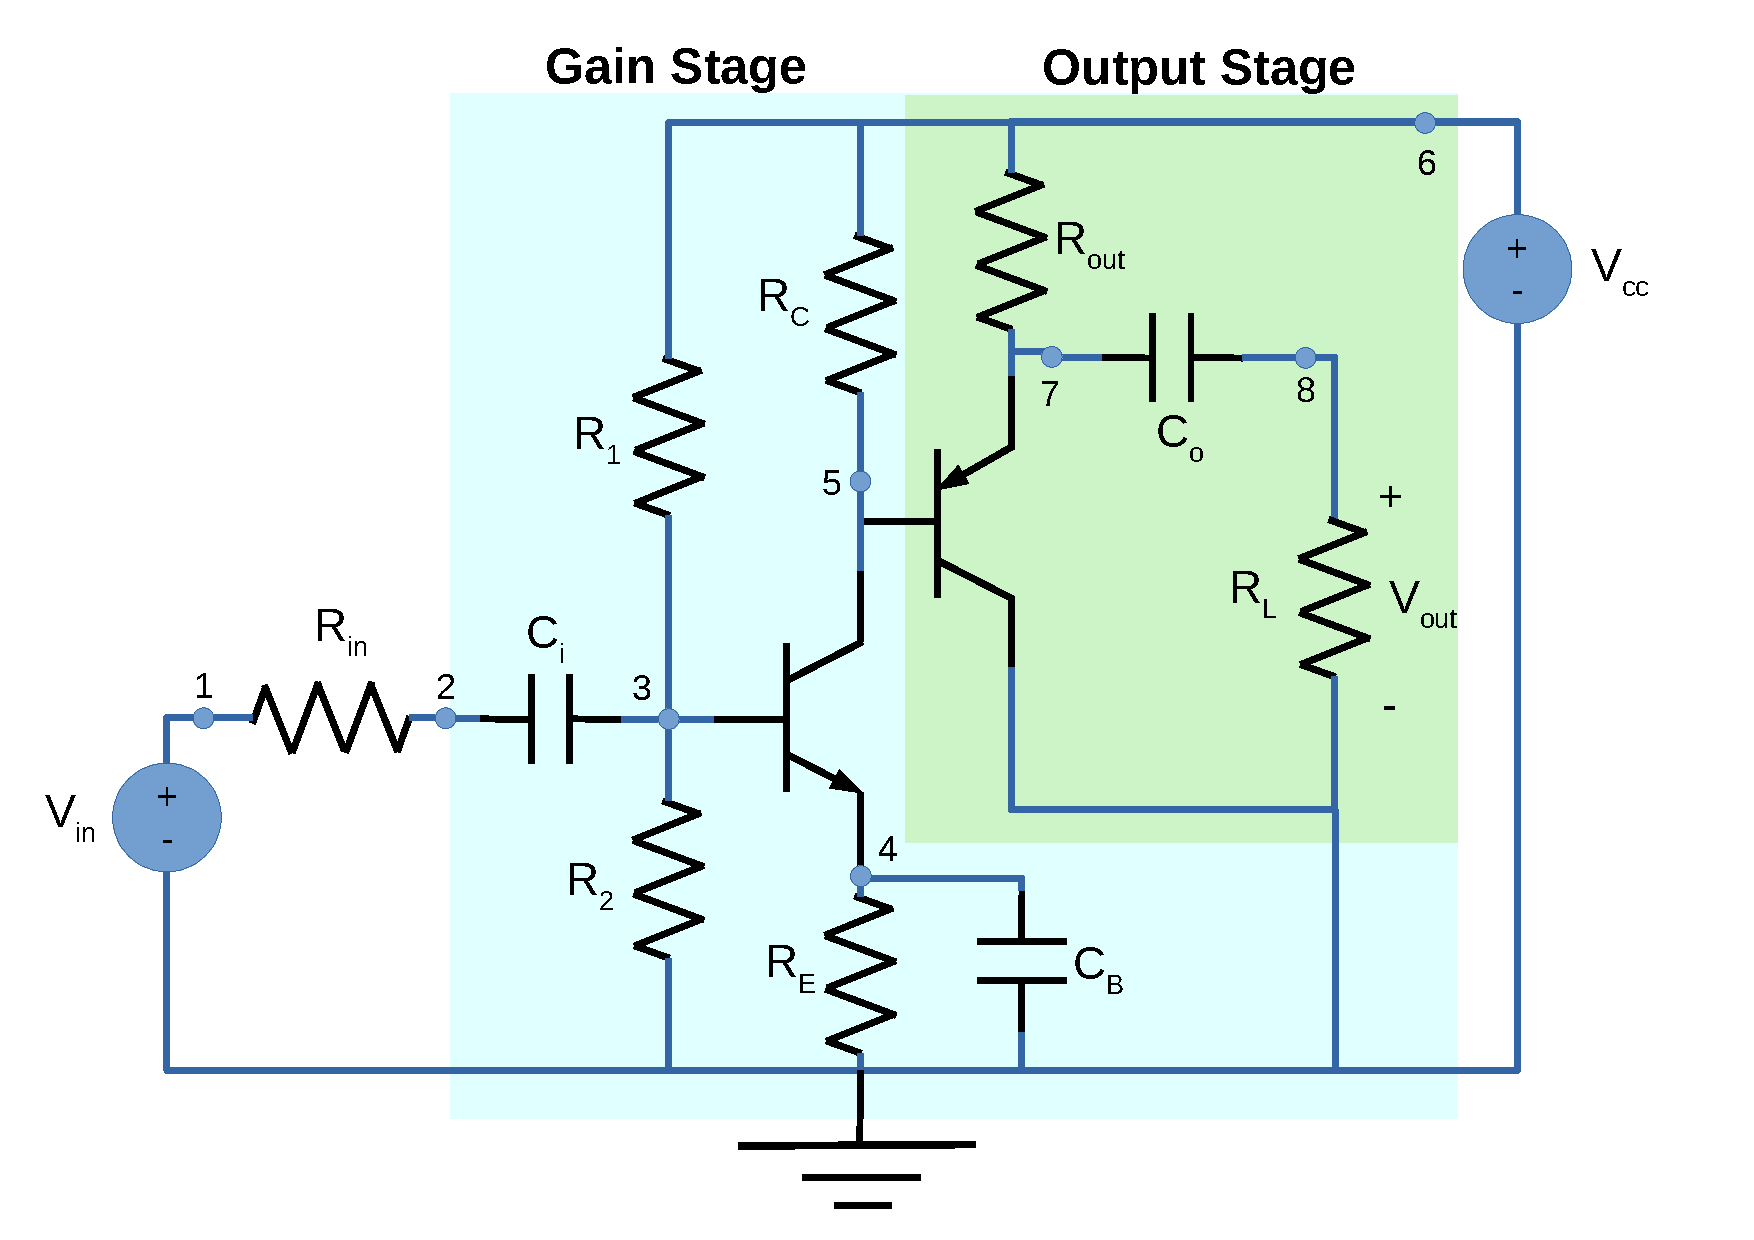
\includegraphics[width = 0.85\linewidth]{scheme.pdf}
            \caption{\textit{Circuit analysed. The fixed values are $V_{in}$ at $10mV$, being of any frequency from $0$ to $10^8$ $Hz$, $V_{cc}$ at $12V$ and the two resistors $R_{in}$ with $100\Omega$ and $R_L$ with $8\Omega$.}}
    \label{fig:bigscheme}
\end{figure}

The results were obtained through a theoretical analysis, in which one predicted the output by using a theoretical method that suited the real circuit and through a simulation that was made using \textit{Ngspice}. The results obtained through both methods will be analysed throughout the report. However, because the models used in \textit{Ngspice} are more correct than the ones used on the theoretical analysis, any type of optimization was done almost exclusively in the simulation analysis\\